\chapter{Results and Discussion}
\label{cha:result}
In this section we apply techniques introduced in \cref{cha:methodology} to test our new methods for nefarious router classification. We present results of nefarious router classification under assumption sets one, two, and three in \cref{ssec:Ras1,ssec:Ras2,ssec:Ras3} respectively. We summarise our findings and comparisons between classifier in \cref{ssec:Rnefidsummary}. Comparisons focus on classifiers two and three as classifier one uses delay distributions not obtainable with network tomography.\par
In \cref{sec:Rprobingoptimality} we present results from testing of candidate optimisation of probe allocation and metric normalisation. Additionally, in \cref{ssec:Rloweraccuracybounds} we calculate the lower bound on the accuracy of each probe allocation scheme for each topology, comparing this to results seen in experimental analysis. Validation of model correctness with respect to assumptions regarding queue length stabilisation, noted as a requirement in previous work, is presented in Appendix A.

\section{Identifying Nefarious Behaviour}
\label{sec:Rnefarouterdetection}
For numerical analysis of classification under our proposed three assumption sets we consider the Nobel, Free, and CPLEX network topologies. This allows us to provide a robust analysis of analytical results using confusion matrices for each classification scenario. For each assumption set we discuss the classifiers performance under each scenario and provide generalised evaluations of each classifier, begin with assumption set one.

\subsection{Classifier One}
\label{ssec:Ras1}
Firstly we consider classification with a full delay distribution and baseline comparisons. Confusion matrices for nefarious router classification are shown in \cref{tab:ngercmatrix,tbl:frncecmatrix,tbl:nrwycmatrix}. Each classification was performed using a KS comparison against the true baseline values and a p-val cutoff of 0.0 to provide the strictly possible guarantee of significance.\par
\noindent
\begin{table}[H]
    \centering
    \aboverulesep = 0pt
    \belowrulesep = 0pt
    \begin{tabular}{l|cc}
        {\backslashbox{\textit{Actual}}{\textit{Predicted}}} & {Nefarious} & {Non-nefarious}\\
        \midrule
        {Nefarious}     & 1807  & 0     \\
        {Non-nefarious} & 37    & 3018  \\
    \end{tabular}
    \caption{Confusion matrix for classification under assumption set 1 in the Nobel topology.}
    \label{tab:ngercmatrix}
\end{table}
\noindent
\begin{table}[H]
    \centering
    \aboverulesep = 0pt
    \belowrulesep = 0pt
    \begin{tabular}{l|cc}
        {\backslashbox{\textit{Actual}}{\textit{Predicted}}} & {Nefarious} & {Non-nefarious}\\
        \midrule
        {Nefarious}     & 2781  & 101     \\
        {Non-nefarious} & 101    & 2658  \\
    \end{tabular}
    \caption{Confusion matrix for classification under assumption set 1 in the Free topology.}
    \label{tbl:frncecmatrix}
\end{table}
\noindent
\begin{table}[H]
    \centering
    \aboverulesep = 0pt
    \belowrulesep = 0pt
    \begin{tabular}{l|cc}
        {\backslashbox{\textit{Actual}}{\textit{Predicted}}} & {Nefarious} & {Non-nefarious}\\
        \midrule
        {Nefarious}     & 1905  & 46     \\
        {Non-nefarious} & 413   & 1896   \\
    \end{tabular}
    \caption{Confusion matrix for classification under assumption set 1 in the CPLEX topology.}
    \label{tbl:nrwycmatrix}
\end{table}
Classification in the Nobel topology has a sensitivity of 100\% across all evaluated sets of nefarious routers. With 37 false positives the classifier has a specificity of 99.99\%, giving an extremely precise and accurate nefarious router classification. For the Free and CPLEX topologies we observe marginally worse classification performance. The classifier has a sensitivity of 96.5\% and 97.64\% and a specificity of 96.34\% and 82.11\% for Free and CPLEX respectively. Therefore, classification in each topology easily meets the 0.9 sensitivity threshold for scenario one.\par
For scenario two, the classifier fulfils the requirements over each topology, achieving a true positive rate >> 0.7. The highest false positive rate occurs in the CPLEX topology where a rate of 0.18 is achieved. Similarly, the classifier meets requirement in scenario three in all topologies. The highest false positive rate occurs in the CPLEX topology at only 0.02.\par
However, the most striking result is a sensitivity of 100\% in the Nobel topology, closely followed by the 99.9\% specificity in the same topology. We anticipate the extreme efficacy of this classification is due to the relatively small number of routers within the Nobel topology allowing us to obtain router identifiability using only 28 probe paths.\par
The larger size, and therefore complexity, of the network means that router queue buffer metrics have more noise. This is due to the number of paths background traffic can take between switches exponentially increasing with network size. In combination with the stochastic routing behaviour, this results in increased noise in the measurements of each router's PDA. We would however expect the true sensitivity of the classifier to however be <100\% but the sample size needed to determine this would be prohibitively large.\par
In all topologies we observe the classifier having a higher sensitivity than specificity. This is likely due to the stochastic routing behaviour of the network routing packets away from nefarious routers which will have larger buffer queues. This would cause non-nefarious routers to receive more packets and subsequently a larger buffer queue, appearing nefarious. Nefarious routers however - even when forwarded few packets - will still delay a proportion of these packet. These routers will therefore maintain a larger queue length, enabling their classification from packet delay metrics and minimising false negatives.\par

\subsection{Classifier Two}
\label{ssec:Ras2}
Next we consider classification with a baseline comparison and only packet delay summary statics available. ROC curves for classification in each topology are given in \cref{fig:RA2ROCcurves}. Note the performance of the classifier under each case is extrapolated from a corresponding point lying on the ROC curve.\par
For scenario one router classification in the Nobel, Free, and CPLEX topologies satisfied the sensitivity threshold of 0.9 with a false positive rate of 0.811, 0.838, and 0.919 respectively. Classification in the Nobel and Free topologies is superior to random classification of routers. However, with a sensitivity of > 0.763 the classification accuracy for the CPLEX network is worse than random. This is due to a sympathetic increase between non-nefarious router PDA (over baseline PDA) and nefarious router PDA. The sympathetic increase is caused by the link-state protocol routing packets around nefarious routers as their buffer queue's fill. This results in more packets being forwarded to non-nefarious routers over the baseline simulation, increasing the difference in PDA from the baseline simulation.\par
For scenario two the classifier reaches the 0.7 sensitivity threshold in the Nobel and Free within the specificity requirement. However, in the CPLEX topology, the specificity requirement is not and the classifier can only achieve a false positive rate of 0.669. For scenario three the 0.9 specificity threshold is satisfied with a false negative rate of 0.558, 0.682, and 0.864 for each topology respectively.\par
In both scenario two and three all classifier perform better than a random classification. However for scenario two classification in the CPLEX topology is notably worse than the Nobel and Free topologies, even when accounting for the increased number of routers. We anticipate this is caused by the same factors as in classifier one. In general though, the less stringent sensitivity requirements reduce the impact of noise on classification.\par
With scenario three's requirements on specificity, the reduction in classifier accuracy is proportional to the number of routers in each topology. Additionally, across all topologies, the classifier performs the best relative to a random classification in sensitivity and specificity ranges of [0.2, 0.76] and [0.24, 0.83] respectively. Classification under assumption case two is therefore better suited to use cases with a higher tolerance for false negatives.\par
\noindent
\begin{figure}[H]
    \centering
    \begin{subfigure}{0.475\textwidth}
        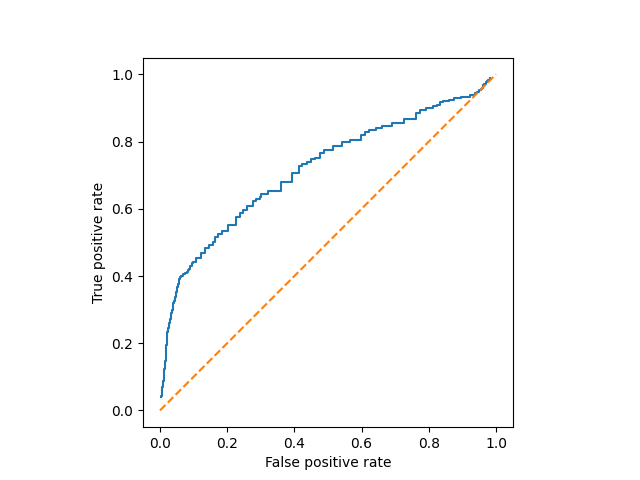
\includegraphics[width=\textwidth]{figs/results/nobel-germany_case2_roc.png}
        \caption{Nobel Topology.}
    \end{subfigure}
    \begin{subfigure}{0.475\textwidth}
        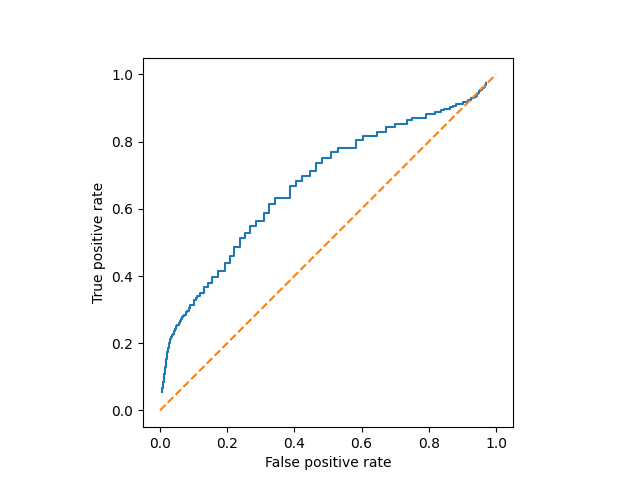
\includegraphics[width=\textwidth]{figs/results/france_case2_roc.png}
        \caption{Free Topology.}
    \end{subfigure}
    \begin{subfigure}{0.475\textwidth}
        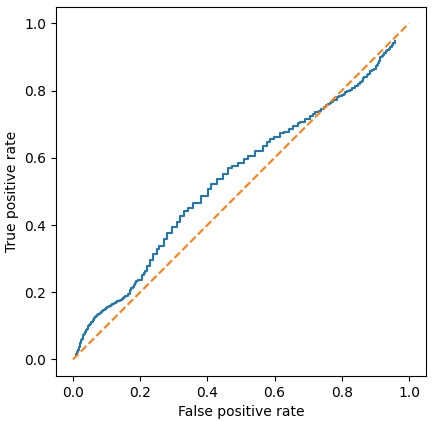
\includegraphics[width=\textwidth]{figs/results/norway_case2_roc.png}
        \caption{CPLEX Topology.}
    \end{subfigure}
    \caption{ROC curves for classification under assumption set 2.}
    \label{fig:RA2ROCcurves}
\end{figure}

\subsection{Classifier Three}
\label{ssec:Ras3}
\noindent
\begin{figure}
    \centering
    \begin{subfigure}{0.475\textwidth}
        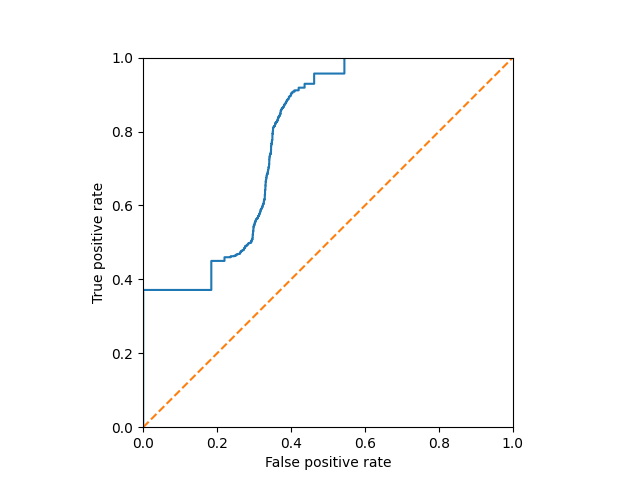
\includegraphics[width=\textwidth]{figs/results/nobel-germany_case3_roc.png}
        \caption{Nobel Topology.}
    \end{subfigure}
    \begin{subfigure}{0.475\textwidth}
        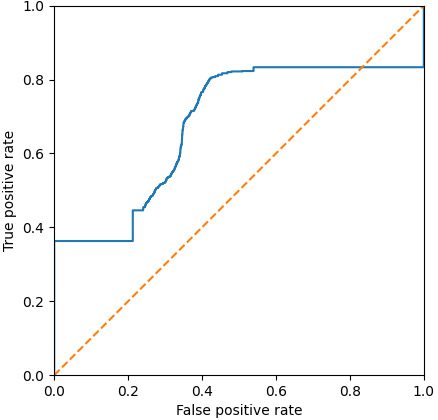
\includegraphics[width=\textwidth]{figs/results/france_case3_roc.png}
        \caption{Free Topology.}
    \end{subfigure}
    \begin{subfigure}{0.475\textwidth}
        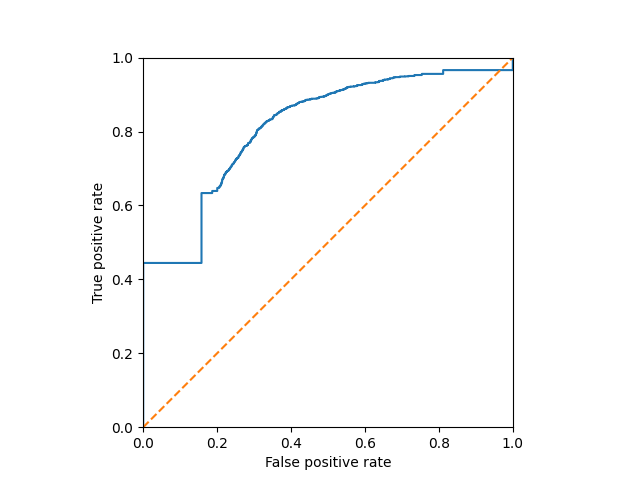
\includegraphics[width=\textwidth]{figs/results/norway_case3_roc.png}
        \caption{CPLEX Topology.}
    \end{subfigure}
    \caption{ROC curves for classification under assumption set 3.}
    \label{fig:RA3ROCcurves}
\end{figure}
Finally we use only packet delay summary statics for classification. ROC curves for classification in each topology are given in \cref{fig:RA3ROCcurves}. We evaluate the classifiers performance for each scenario below.\par
For scenario one classification of the Nobel and CPLEX topologies results in a false positive rate of 0.4 and 0.5 respectively. For the Free topology the classifier is only able to attain a sensitivity of 0.9 with a false negative rate of 1.0 (classify all routers as nefarious). Excluding this case, PDA is not sufficient to classify routers with a sensitivity greater than 0.83 in the Free topology.\par
This is due to the topology containing a router with a degree of 10 (this router represents the city of Paris). The Paris router experiences more than twice as much traffic as the average router of degree 3 and thus has a near or completely full queue buffer regardless of nefarious behaviour. This is compounded by 15 of the 37 probe paths including Paris, resulting in a disproportionate number of probe packets traversing the router. Therefore when using a PDA threshold of buffer queue length $-\epsilon$ for classification the Paris router is always classified as nefarious. A similar limitation exists in the CPLEX topology where due to the same factors where a maximum sensitivity of 0.966 can be achieved.\par
Conversely, the classifier performs extremely well on the Nobel topology achieving a true positive rate of 1.0 with a false positive rate of 0.544. Although both Nobel and CPLEX have a maximum router degree of 6, in the Nobel network only 12 probe paths traverse the maximally connected router compared to 21 in CPLEX. Therefore in the CPLEX network, unlike the Free network, the maximally connected router's buffer queue receives disproportionately more probe packets. This results in the router being classified as nefarious regardless of its delaying behaviour in the majority of test trials.\par
For scenario two classification of all topologies meets specificity and sensitivty requirements. Classification in the Nobel, Free, and CPLEX topologies at the false negative threshold have a false positive rate of 0.339, 0.363, and 0.235 respectively. These rates are a strict improvement over those from classifier two. This improvement is due to the increased queue length of nefarious routers causing traffic to be re-routed through non-nefarious routers, increasing their queue lengths. As this sympathetic increase is absent in the baseline simulation, an increase in PDA is seen from non-nefarious router's baseline. This increase is indistinguishable from the buffer queue increase in nefarious routers. Therefore, there we observe more cases of routers being incorrectly labeled as nefarious.\par
For scenario three classification of each topology results in a false negative rate of 0.629 for the Nobel and Free topologies and 0.556 for CPLEX. However, for each case in \cref{fig:RA3ROCcurves} no PDA thresholds enable a classification with a false positive rate < 0.2. This is due to an overlap in PDA values between weakly connected nefarious router and strongly connected non-nefarious routers. The amount of traffic arriving at strongly connected non-nefarious routers fills their buffer queue at a rate similar to a less connected nefarious router. Therefore, any PDA threshold sufficient to identify any weakly connected nefarious routers incorrectly labels strongly connected non-nefarious routers.\par
We note that as the PDA of each router is dependant on it's queue buffer length, the accuracy of this classifier would suffer severely in network with heterogeneous router buffer queue lengths. The assumption around router homogeneity is however reasonable as for at-scale data center and ISP networks environments homogeneity is maintained. ALthough, for smaller scale at ad hoc home hobby networks or IoT networks where heterogeneity in networking components is far more likely this could present an issue. 

\subsection{Summary of Comparisons}
\label{ssec:Rnefidsummary}
In this section we have analysed three nefarious routers classifiers with three real-world use cases for a fair comparison of performance. Classifier one was found to have the best performance in each use case. This classifier achieved a near perfect accuracy across all investigated topologies. However, as this underlying distribution can not be obtained via network tomography we focused our comparison on the second and third classifiers.\par
Classifier two was found to perform better than a random classification in all cases other than in the CPLEX topology with a sensitivity > 0.763. This was caused by a sympathetic increase between non-nefarious router PDA (over baseline PDA) and nefarious router PDA due to stochastic traffic routing. This classifier performed optimally for specificity requirements between 0.24 and 0.83 across all topologies.\par
Classifier three achieved greater accuracy than classifier two for sensitivity and specificity requirements of [0.2, 0.83] and [0.46, 0.75] respectively. This was due to absence of baseline comparisons causing sympathetic increases between routers to not impact classification. However, classifier two performed very poorly for sensitivities below 0.2 and above 0.8. This was due to an overlap in PDA metrics between strongly connected non-nefarious and weakly connected nefarious.

\section{Optimisation Impacts}
\label{sec:Rprobingoptimality}
In this section we apply optimisations to the allocation of probe packets between probe paths and metrics collected from this probing. Classification resulting from these candidate optimisation are compared and contrasted to original measures to quantify their impact.\par
In \cref{ssec:Rprobeallocation} we present ROC curves to evaluate performance of classifiers two and three using a proportional probe allocation (PPA). We discuss the performance of each classifier for each real-world topology. In \cref{ssec:Rloweraccuracybounds} we then compute the CRB for each probe allocations scheme in each topology. The CRB bounds are then compared to ROC curves for both probing schemes in each topology. Additionally, we contrast the CRB for each topology, discussing the impact of the number of routers in each network on this lower accuracy bound.\par
In \cref{ssec:Rmetricnormilisation} we present results from classification with each router's PDA normalised w.r.t. the router's degree. The produced ROC curves for classifier two and three in each topology are compared to baseline results without this normalisation.

\subsection{Proportional Probe Allocation}
\label{ssec:Rprobeallocation}
In \cref{fig:RprobeoptROCcurves} we present results from classification with PDA inferred from network tomography. Sub-figures (a), (c), and (e) correspond to classifier two and sub-figures (b), (d), and (f) correspond to classifier three. Classifier one is not included in our analysis here as the information it requires cannot be obtained via network tomography. In each sub-figure a ROC curve showing classification accuracy is provided for both unoptimised and optimised PPA over paths.\par
Using a two-sample Kolmogorov–Smirnov test we evaluate the distribution of true positives for each classifier in each topology, results are shown in \cref{tbl:Roptkstest}. Given our average is taken over 50 simulations we select an generally accepted p-value of 0.05 to indicate a significant improvement. From this we can reject the null hypothesis of the sensitivity distribution under an equal probe allocation compared to PPA for classifier two in the Nobel and CPLEX topologies and classifier three in the Nobel topology. In each of these PPA results in a mean sensitivity improvement of 0.214, 0.1, and 0.204 respectively over all false positive rates.\par
This means that for any set maximal tolerance of false positive we are on average able to correctly classify 17\% more nefarious routers using network tomography with PPA. Note that improvements can also be seen in sub-figure f where PPA enables classification with a minimum false positive rate of 5\% compared to only 50\% without optimisation. This is, however, not reflected in p-value test results as the comparison is only computed for sensitivity.\par
\noindent
\begin{figure}[H]
    \centering
    \begin{subfigure}[H]{0.475\textwidth}
        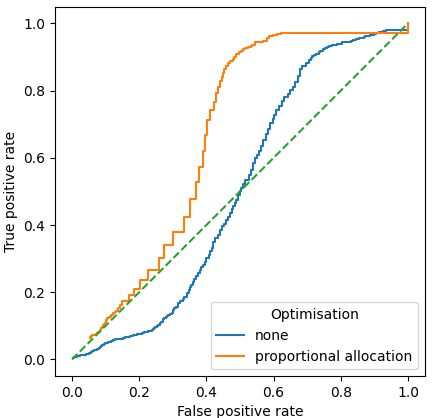
\includegraphics[width=\textwidth]{figs/results/nobel-germany_ac2_opt.png}
        \caption{Nobel topology with classifier 2.}
    \end{subfigure}
    \begin{subfigure}[H]{0.475\textwidth}
        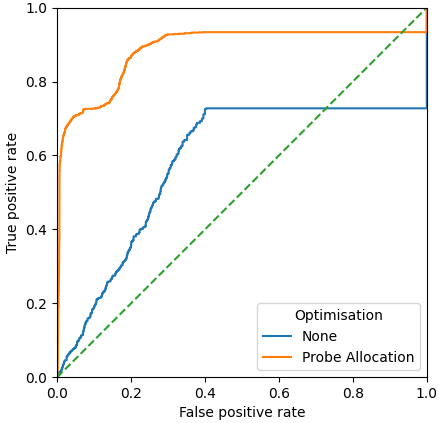
\includegraphics[width=\textwidth]{figs/results/nobel-germany_ac3_opt.png}
        \caption{Nobel topology with classifier 3.}
    \end{subfigure}
    \begin{subfigure}[H]{0.475\textwidth}
        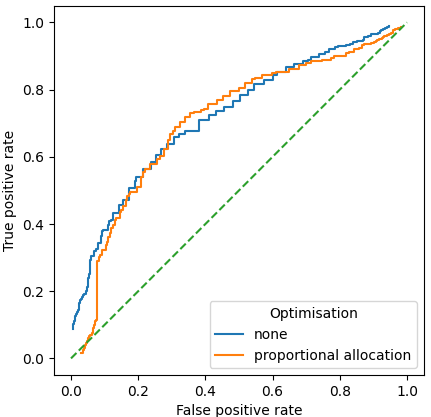
\includegraphics[width=\textwidth]{figs/results/france_ac2_opt.png}
        \caption{Free topology with classifier 2.}
    \end{subfigure}
    \begin{subfigure}[H]{0.475\textwidth}
        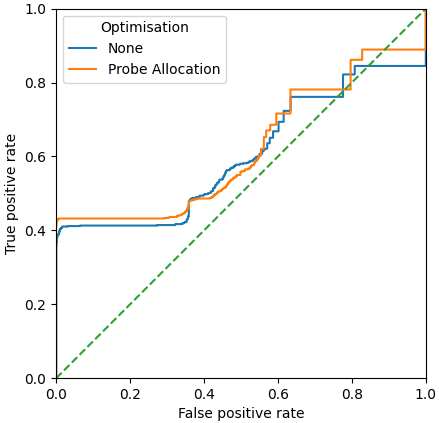
\includegraphics[width=\textwidth]{figs/results/france_ac3_opt.png}
        \caption{Free topology with classifier 3.}
    \end{subfigure}
    \begin{subfigure}[H]{0.475\textwidth}
        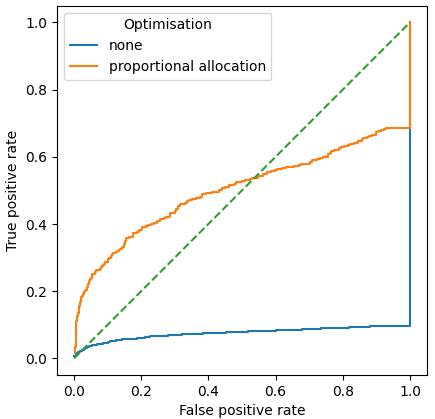
\includegraphics[width=\textwidth]{figs/results/norway_ac2_opt.png}
        \caption{CPLEX topology with classifier 2.}
    \end{subfigure}
    \begin{subfigure}[H]{0.475\textwidth}
        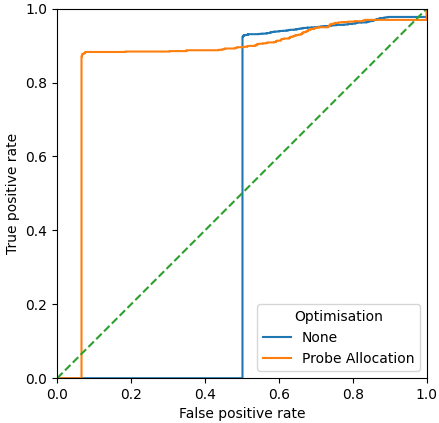
\includegraphics[width=\textwidth]{figs/results/norway_ac3_opt.png}
        \caption{CPLEX topology with classifier 3.}
    \end{subfigure}
    \caption{ROC curves for optimised classification.}
    \label{fig:RprobeoptROCcurves}
\end{figure}

\begin{table}[H]
 \centering
  \begin{tabular}{@{}ccc@{}}
   \toprule
    Topology & Classifier & KS test P-value \\
    \midrule
    Nobel & 2 & 1.08e-06\\
    Nobel & 3 & 0\\
    Free  & 2 & 0.619\\
    Free  & 3 & 0.280\\
    CPLEX & 2 & 4.31e-57\\
    CPLEX & 3 & 1.00\\
   \bottomrule
  \end{tabular}
  \caption{Calculated Cramér–Rao bound for each topology and probe allocation}
  \label{tbl:Roptkstest}
\end{table}
This improvement in classifier performance with PPA for the Nobel and CPLEX topologies is due to the variation of routers between probe paths. For both the Nobel and CPLEX topologies a single router is present in at most 25\% of paths however in the Free topology a single router is present in at most 47\% of probe paths. This means that, with a proportion allocation, this singular router in the Free topology receives disproportionately more packets. Many of these additional probe packets are dropped due to the limited queue buffer, resulting in only minor changes in classification accuracy from the PPA.\par
In sub-figure (a), for false positive rates < 0.5 classification with unoptimised probe allocation is worse than random. This result is unlikely to be due to noise as it has been average over many simulation runs. We speculate that this poor classification is potentially due to the buffers of nefarious routers being comprised of solely probe packets. This could potentially be caused by traffic re-routing around these nefarious routers. PDA measurements would therefore be far lower than would be expected if background traffic was also being forwarded to these routers. However, additional investigation into this behaviour in future work is required to form a substantiated explanation.

\subsection{Cramér–Rao Bounds}
\label{ssec:Rloweraccuracybounds}
Results from analytical calculation of the CBR given probe paths and probe allocation for each topology are given in \cref{tbl:crbs}. In each case the CRB is extremely low, this is due to the large number of probe paths used in tomography for each topology. However, as this only represent a lower bound we focus on comparison of the CRB between topologies and each probe allocation scheme in a topology.\par
For both probe allocations network tomography in the Nobel topology has the highest CRB. Probing the in the Free and CPLEX topologies was calculated to have the second highest and lowest CRB respectively. This corresponds to classifier accuracy evaluation from ROC curves of each classifier in \cref{fig:RprobeoptROCcurves}. This decrease in accuracy is proportional to the increase in number of routers in each each topology. This is due to the additional probe paths required to uniquely identify each router reducing the number of measurements we are able to take over each path.\par
However, under PPA probing the larger CPLEX network has a higher CRB than the Free network. This is due to the Free topology containing a router with a degree of ten which a disproportionate number of probe paths traverse. Under PPA more probe packets are sent to this router, causing more to be dropped as its buffer queue is already at capacity. These dropped probe packets are the cause of this decrease in the lower accuracy bound.\par
Comparing probing scheme within topologies, the CRB of network tomography with PPA is greater than with an unoptimised probe allocation for each topology. The improvement in accuracy of network tomography in the Nobel and CPLEX topologies is 2.07e-4 and 7.92e-6, however, for the Free topology the improvement is only -4.9e-7.\par
\begin{table}[H]
 \centering
  \begin{tabular}{@{}ccc@{}}
   \toprule
    &\multicolumn{2}{c}{\textbf{Probe Allocation}}\\
    \cmidrule(rl){2-3}
    Topology & Unoptimised & PPA \\
    \midrule
    Nobel & 3.18e-05 & 2.39e-04\\
    Free & 1.42e-06 & 1.91e-06\\
    CPLEX & 1.94e-07 & 8.11e-06\\
   \bottomrule
  \end{tabular}
  \caption{Calculated Cramér–Rao bound for each topology and probe allocation}
  \label{tbl:crbs}
\end{table}
This is consistent with ROC curves in \cref{fig:RprobeoptROCcurves} where a significant improvement in classification was observed for the Nobel and CPLEX topologies. Additionally, the smaller difference in CRB between probe allocation schemes for the Free topology corresponds with classifier performance, where the smallest difference between probe allocation schemes was observed.\par


\subsection{Metric Normalisation}
\label{ssec:Rmetricnormilisation}
ROC curves for nefarious router classification with PDA normalised w.r.t. router degree are shown in \cref{fig:RmetricnormROCcurves}. We omit classifier one as it does not use PDA for classification. For classifier two, a decrease in accuracy across all true and false positives rates is seen. Similarly, for classifier three an equal or lesser accuracy over all topologies is seen.\par
The general decrease in classification accuracy is likely due to a router's degree being a poor representation of the number of packets it receives each timestep. Other contributing factors such as the routing tables of surrounding routers and their respective degree would also likely need to be accounted for. It is also possible that the contributions of incoming traffic and nefarious delaying to a routers queue length are intrinsically related.\par
This would mean that attempts to account for incoming traffic contributions to better identify nefarious delaying are unlikely to yield classification improvements irrelevant of the number of factors relating to incoming traffic volume are accounted for. We therefore highlight methods of distinguishing between incoming traffic, and other factors which contribute to a router's buffer queue size, to better identify nefarious delaying behaviour as an area for future research.\par
\noindent
\begin{figure}[H]
    \centering
    \begin{subfigure}[H]{0.475\textwidth}
        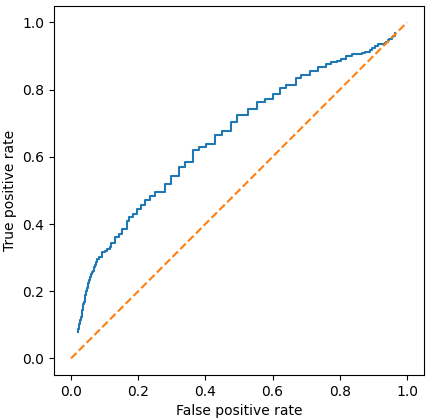
\includegraphics[width=\textwidth]{figs/results/metric_normilisation/nobel-germany_ac2.png}
        \caption{Nobel Topology Classifier 2.}
    \end{subfigure}
    \begin{subfigure}[H]{0.475\textwidth}
        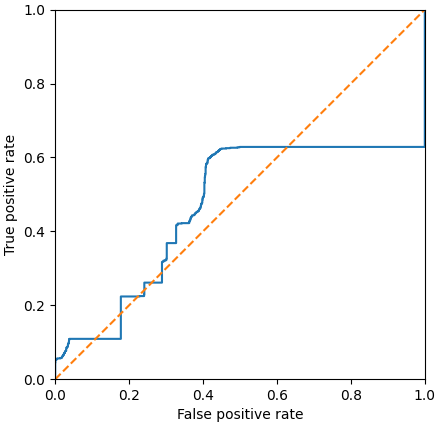
\includegraphics[width=\textwidth]{figs/results/metric_normilisation/nobel-germany_ac3.png}
        \caption{Nobel Topology Classifier 3.}
    \end{subfigure}
    \begin{subfigure}[H]{0.475\textwidth}
        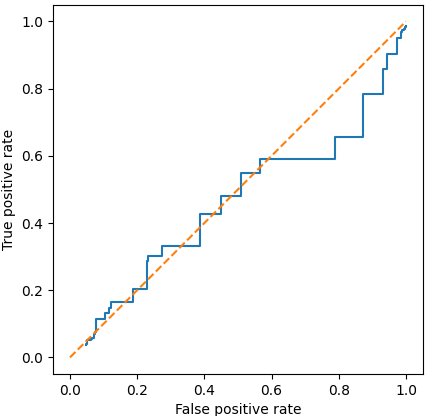
\includegraphics[width=\textwidth]{figs/results/metric_normilisation/france_ac2.png}
        \caption{Free Topology Classifier 2.}
    \end{subfigure}
    \begin{subfigure}[H]{0.475\textwidth}
        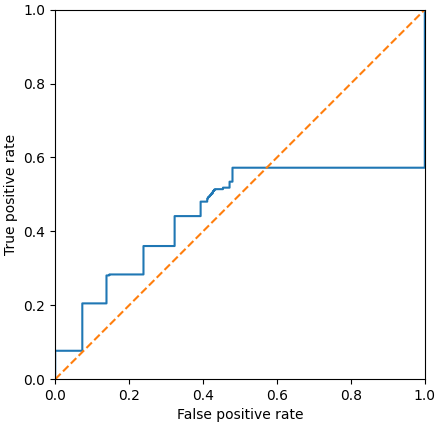
\includegraphics[width=\textwidth]{figs/results/metric_normilisation/france_ac3.png}
        \caption{Free Topology Classifier 3.}
    \end{subfigure}
    \begin{subfigure}[H]{0.475\textwidth}
        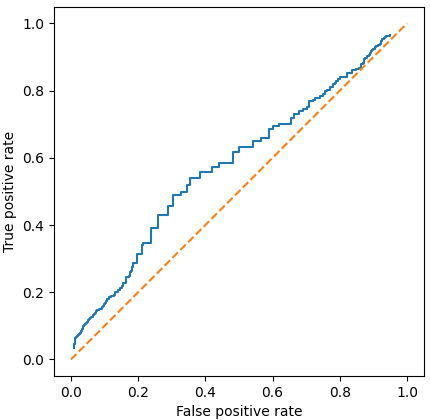
\includegraphics[width=\textwidth]{figs/results/metric_normilisation/norway_ac2.png}
        \caption{CPLEX Topology Classifier 2.}
    \end{subfigure}
    \begin{subfigure}[H]{0.475\textwidth}
        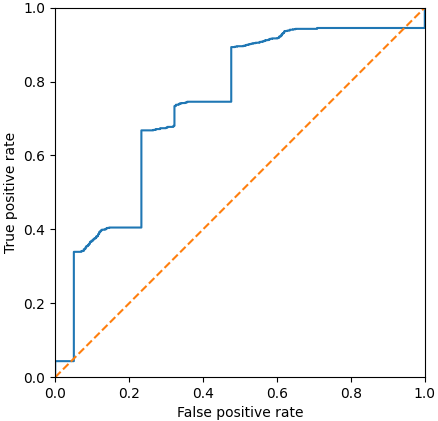
\includegraphics[width=\textwidth]{figs/results/metric_normilisation/norway_ac3.png}
        \caption{CPLEX Topology Classifier 3.}
    \end{subfigure}
    \caption{ROC curves for optimised classification.}
    \label{fig:RmetricnormROCcurves}
\end{figure}

\section{Summary}
In this chapter we have presented experimental results of three classifiers of nefarious router behaviour in three real world ISP topologies. The efficacy of each classifier was discussed and comparison between each classifier were made. Classifier one was found to be the most effective. Confusion matrices for classifier one's performance on each topology were presented and a small decrease in classifier performance was seen for topologies with more routers.\par
For classifier two and three ROC curves were produced, varying the threshold for a router to be labeled as nefarious. Three use cases corresponding to the upper left, middle, and lower right segments of the ROC curve were used to compare classifier two and three. These three segments of the ROC curve correspond to varying specificity and sensitivity requirements.\par
Classifier two was found to be more effective than classifier two at identifying nefarious routers when a high specificity or sensitivity was required. This was due to the comparison to baseline router metrics used allowing for a finer grained distinction of router performance to be made. In contrast, Classifier three was unable to distinguish between nefarious and non-nefarious router with a very high specificity or sensitivity. This was due to overlap in the PDA of strongly connected non-nefarious routers and weakly connected nefarious routers.\par
However, classifier three was found to more effective at identifying nefarious routers at the centre of the ROC curve where less stringent specificity and sensitivity requirements were required. This was due to a sympathetic increase in non-nefarious router PDA over baseline measurements due to background traffic be re-routed to these non-nefarious routers. Using PDA alone for identification, classifier two was unaffected by this sympathetic increase. Classifier three was therefore able to more effectively label nefarious nodes in cases where there was no overlap between nefarious and non-nefarious router PDA.\par
Following this, candidate optimisations to probe packet allocation and metric normalisation were analysed. Results using classifier two and three on PDA data from network tomography with and without proportional probe allocation (PPA) were presented in ROC curves. Improved classifier performance was observed in the Free and CPLEX topologies when using PPA. However, classifier two with unoptimised probing was found to perform worse than a random classification for false positive rates less than 0.5 in the Nobel topology. We anticipate this may have been due to background traffic not being routed through nefarious routers, causing their buffer queues to consist of only probe packets.\par
Additionally, performance of classifier two and three in the Free topology was relatively unaffected by the use of PPA in network tomography. This was due to a higher portion of probe paths traversing a common router in the Free topology, causing this router's queue buffer to reach capacity and drop probe packets. Proportional allocation when sending probes therefore did not impact the number of probes received by the destination monitors in each probe path, nullifying any impacts from PPA.\par
The Cramér–Rao bound of both probing schemes in each topology was then calculated and contrasted against the observed performance of each classifier. The CRB was found to be very low in all cases due to the number of probe paths required in each topology. However, the CRB was found to corroborate observed classifier performance both between topologies and between probing schemes over the same topology.\par
Finally we analysed the impact of normalising PDA measurements w.r.t. the degree of each router. This was done to account for the contribution of incoming traffic to the size of each router's queue buffer. However, performance of classifier two and three was found to be worse with this metric normalisation for every topology considered. We postulated that this was due to a router's degree being insufficient to account for the contribution of incoming traffic to the size of its queue buffer. We also discussed the possibility that the factors contributing to a router's queue buffer size are intrinsically related and no amount of data post-processing can better identify the contribution of nefarious delaying.